%----------------------------------------------------------------------------
\chapter{Módszertan}
\label{ch:modszer}
%----------------------------------------------------------------------------

\section{Mérésben résztvevő személyek}
A kutatás során 7 igazolt, versenyszerű kosárlabda múlttal rendelkező játékos (6 férfi, 1 nő) bevonásával történt az adatgyűjtés. Kizárólag sérülésmentes sportolók kerültek bevonásra a vizsgálatba. A mérésben résztvevő összes személy jobbkezes volt. A játékosok fizikai paraméterei és tapasztalati szintje részletesen rögzítésre került (lásd \ref{tab:participants}. táblázat). A teljes minta átlagéletkora $20{,}3 \pm 0{,}5$ év, átlagos testmagassága $185{,}8 \pm 7{,}0$~cm, míg átlagos testtömege $82{,}2 \pm 8{,}3$~kg volt. A résztvevők átlagosan $12{,}7 \pm 1{,}3$ év igazolt sportmúlttal rendelkeztek. Az egyes mérések előtt a sportolók adatai rögzítésre kerültek (név, testmagasság, testtömeg, kosárlabdával eltöltött évek száma) és a résztvevők tájékoztatva lettek a mérés menetéről. A résztvevők írásos beleegyezést adtak. A rögzített adatok kizárólag kutatási céllal kerülnek feldolgozásra és azok tárolása a személyiségi jogoknak megfelelően történik. A kutatást a Testnevelési Egyetem Tudományos és Kutatásetikai Bizottsága engedélyezte (TE-KEB/No04/2024).

\begin{table}[!ht]
    \centering
    \caption{A mérésben résztvevő játékosok fizikai és demográfiai adatai. Valamennyi résztvevő jobbkezes volt.}
    \label{tab:participants}
    \begin{tabular}{lcccc}
        \toprule
        \textbf{Nem} & \textbf{Életkor (év)} & \textbf{Testmagasság (cm)} & \textbf{Testtömeg (kg)} & \textbf{Tapasztalat (év)} \\
        \midrule
        Nő           & -                     & -                          & -                       & -                         \\
        Férfi        & 20                    & 180                        & 72                      & 14                        \\
        Férfi        & 19                    & 179                        & 87                      & 14                        \\
        Férfi        & 19                    & 181                        & 73                      & 11                        \\
        Férfi        & 20                    & 186                        & 80                      & 14                        \\
        Férfi        & 20                    & 196                        & 92                      & 11                        \\
        Férfi        & 19                    & 193                        & 89                      & 12                        \\
        \bottomrule
    \end{tabular}
\end{table}

\section{Mérési eszközök és beállítás}
A vizsgálat során a videóalapú pózbecslés mellett egy OptiTrack (NaturalPoint, Inc., Corvallis, OR, USA) típusú 3D optikai mozgáskövető (MoCap) rendszer is alkalmazásra került referenciaként és a gépi tanulási modellek pontosságának növelése érdekében. A felvételek párhuzamosan két okostelefonnal (egy Android és egy iOS rendszerű készülékkel) is rögzítésre kerültek, egységesen 1080p (Full HD) felbontásban és 60 fps (képkocka/másodperc) rögzítési sebességgel. A monokuláris pózbecslő rendszerek sajátossága, hogy nem igényelnek hagyományos 3D kamera kalibrációt, azonban a konzisztencia érdekében a kamerák dőlésszöge és magassága minden felvételnél fixen maradt.

A \ref{fig:camera_setup}. ábra mutatja a mérés elrendezését. A játékos a szabványos büntetővonalon helyezkedett el, míg a kamerák a játékostól balra, illetve jobbra, a gyűrűhöz kissé közelebb eső fix pozíciókban (oldalnézetből) álltak fel, biztosítva, hogy a játékos teljes teste végig a látótérben maradjon. A markerelrendezés pontos anatómiai lokációit a \ref{fig:mocap_markers}. ábra szemlélteti.

\begin{figure}[!ht]
    \centering
    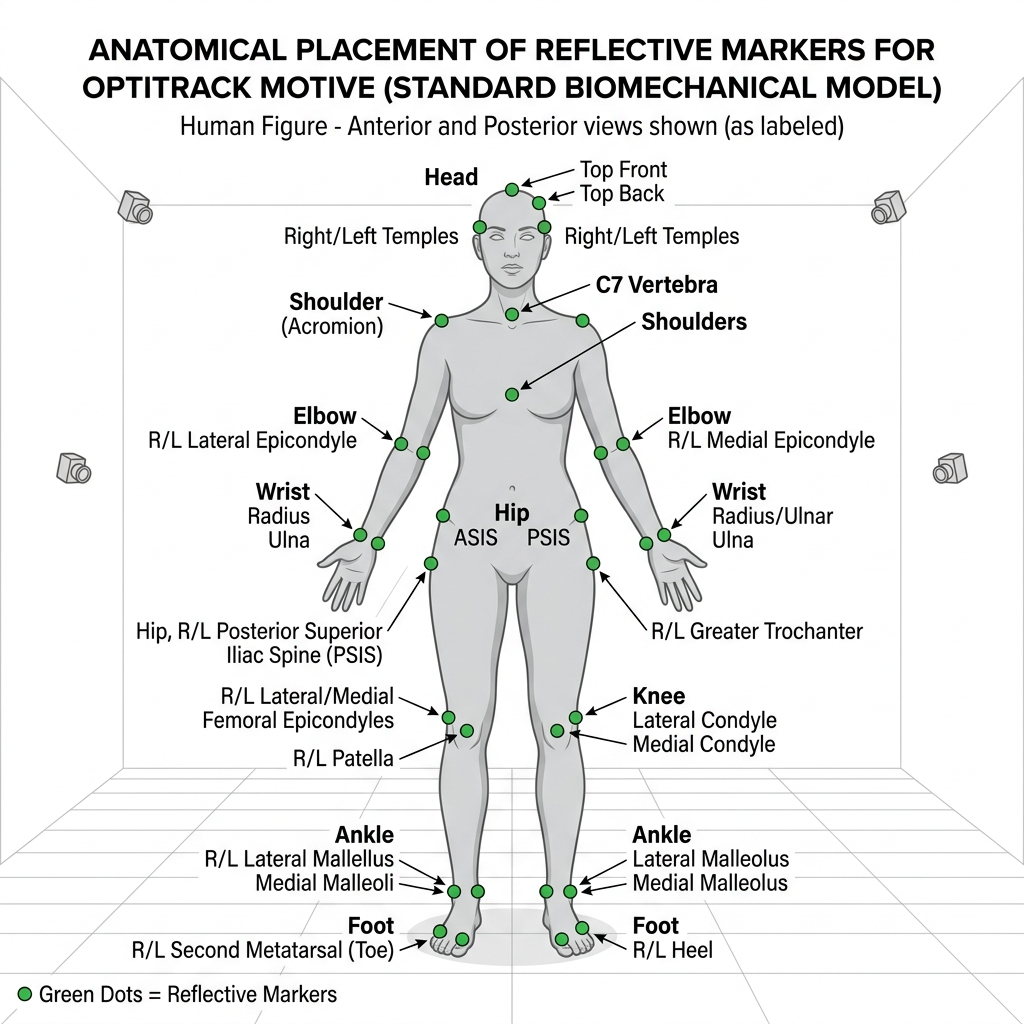
\includegraphics[width=0.7\textwidth, keepaspectratio]{imgs/mocap_markers.png}
    \caption{A fényvisszaverő markerek standard anatómiai elrendezése (OptiTrack Motive szoftverhez).}
    \label{fig:mocap_markers}
\end{figure}

\begin{figure}[!ht]
    \centering
    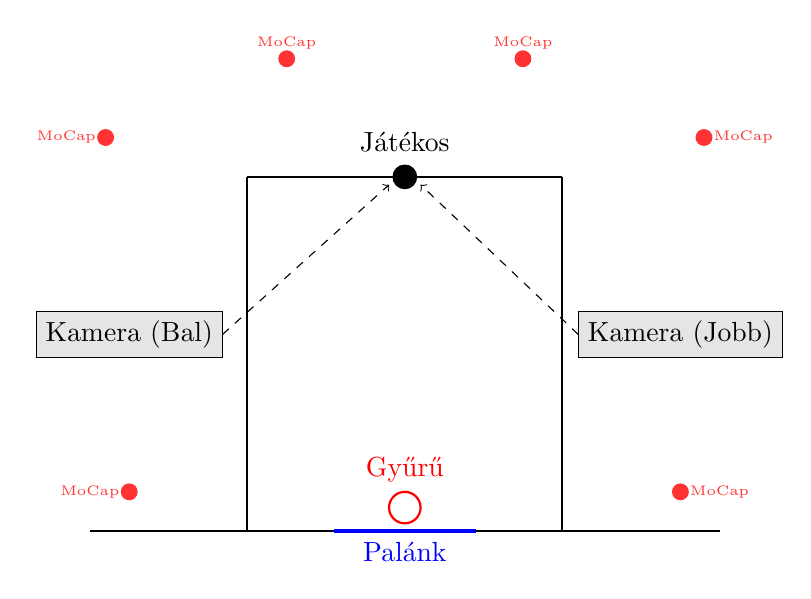
\begin{tikzpicture}
        % Pálya határai (vonalak)
        \draw[thick] (-4, 0) -- (4, 0); % Alapvonal
        \draw[thick] (-2, 0) -- (-2, 4.5); % Büntetőterület bal
        \draw[thick] (2, 0) -- (2, 4.5); % Büntetőterület jobb
        \draw[thick] (-2, 4.5) -- (2, 4.5); % Büntetővonal

        % Gyűrű és palánk
        \draw[ultra thick, blue] (-0.9, 0) -- (0.9, 0) node[midway, below] {Palánk};
        \draw[thick, red] (0, 0.3) circle (0.2) node[above=0.2cm] {Gyűrű};

        % Játékos
        \filldraw[black] (0, 4.5) circle (0.15) node[above=0.2cm] {Játékos};

        % Kamerák (Okostelefonok)
        \node[draw, rectangle, fill=gray!20, minimum width=1cm, minimum height=0.5cm] (camL) at (-3.5, 2.5) {Kamera (Bal)};
        \node[draw, rectangle, fill=gray!20, minimum width=1cm, minimum height=0.5cm] (camR) at (3.5, 2.5) {Kamera (Jobb)};

        % MoCap kamerák (infravörös)
        \filldraw[red!80] (-3.8, 5) circle (0.1) node[left] {\tiny MoCap};
        \filldraw[red!80] (3.8, 5) circle (0.1) node[right] {\tiny MoCap};
        \filldraw[red!80] (-3.5, 0.5) circle (0.1) node[left] {\tiny MoCap};
        \filldraw[red!80] (3.5, 0.5) circle (0.1) node[right] {\tiny MoCap};
        \filldraw[red!80] (-1.5, 6) circle (0.1) node[above] {\tiny MoCap};
        \filldraw[red!80] (1.5, 6) circle (0.1) node[above] {\tiny MoCap};

        % Kamera látószögek
        \draw[dashed, ->] (camL.east) -- (-0.2, 4.4);
        \draw[dashed, ->] (camR.west) -- (0.2, 4.4);

    \end{tikzpicture}
    \caption{A mérés sematikus elrendezése. A piros pontok a MoCap kamerákat, a szürke téglalapok az okostelefonokat jelölik.}
    \label{fig:camera_setup}
\end{figure}

\section{Mérési protokoll}
A videófelvételek valós környezetben, szabványos kosárlabdapályán készültek. A mérést megelőzően a játékosok egy rövid, sportágspecifikus bemelegítést végeztek, amely 3-8 szabadon választott bemelegítő büntetődobásból állt.

Ezt követően minden résztvevő 4 sorozatban hajtott végre 5-5 dobást. A dobások között 5-10 másodperc, míg a sorozatok között 1 perc pihenőidő állt rendelkezésre a fáradás minimalizálása érdekében. Néhány esetben egy-egy sorozatot technikai okok (pl. kitakarás) miatt újra kellett rögzíteni. A felvételeken minden dobás kimenetele (sikeres vagy sikertelen) manuálisan rögzítésre került, amely elengedhetetlen feltétele volt a felügyelt gépi tanulásnak.

\section{Adatfeldolgozás}
A szoftveres adatfeldolgozás során kerültek kinyerésre a biomechanikai paraméterek a videókból. A folyamat lépéseit a \ref{fig:pipeline_flowchart}. ábra szemlélteti.

\tikzstyle{process} = [rectangle, minimum width=3cm, minimum height=1cm, text centered, draw=black, fill=blue!10, rounded corners]
\tikzstyle{arrow} = [thick,->,>=stealth]

\begin{figure}[!ht]
    \centering
    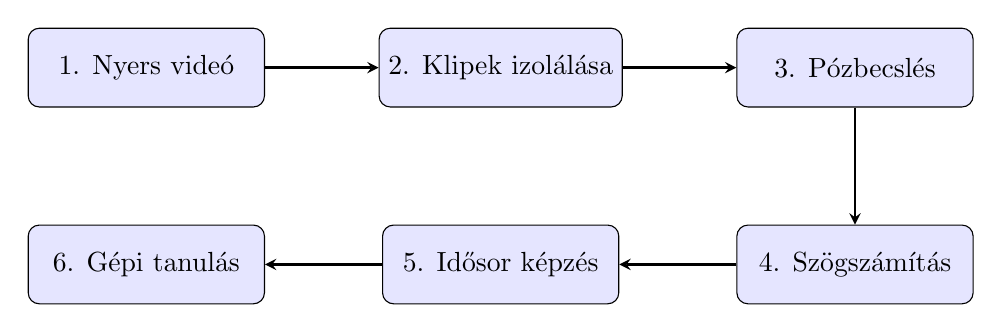
\begin{tikzpicture}[node distance=2cm]
        \node (video) [process] {1. Nyers videó};
        \node (isolate) [process, right of=video, xshift=2.5cm] {2. Klipek izolálása};
        \node (pose) [process, right of=isolate, xshift=2.5cm] {3. Pózbecslés};
        \node (angle) [process, below of=pose, yshift=-0.5cm] {4. Szögszámítás};
        \node (feature) [process, left of=angle, xshift=-2.5cm] {5. Idősor képzés};
        \node (ml) [process, left of=feature, xshift=-2.5cm] {6. Gépi tanulás};

        \draw [arrow] (video) -- (isolate);
        \draw [arrow] (isolate) -- (pose);
        \draw [arrow] (pose) -- (angle);
        \draw [arrow] (angle) -- (feature);
        \draw [arrow] (feature) -- (ml);
    \end{tikzpicture}
    \caption{A biomechanikai adatfeldolgozás automatizált szoftveres folyamatábrája.}
    \label{fig:pipeline_flowchart}
\end{figure}

A nyers videófelvételek első lépésben automatikusan feldarabolásra kerültek, így önálló dobási klipek jöttek létre. A 3. lépésben (Pózbecslés) két különböző marker nélküli algoritmus integrációja történt meg, amelyeket a precízebb elemzés érdekében az OptiTrack rendszerből származó adatok egészítettek ki:
\begin{itemize}
    \item \textbf{YOLO (You Only Look Once):} GPU-ra optimalizált (TensorRT gyorsítással), ami 17 alapvető 2D kulcspontot azonosít.
    \item \textbf{MediaPipe:} 33 darab térbeli (3D) kulcspontot (köztük a kézfej pontjait) határoz meg. CPU-n fut, de párhuzamosítással kellően gyors, és a több referenciapont miatt részletesebb kinematikai elemzést tesz lehetővé.
    \item \textbf{OptiTrack Motive (MoCap):} Marker-alapú rendszer, amely fizikai markerek alapján milliméteres pontossággal követi a csontváz (skeleton) térbeli mozgását. Az adatok feldolgozásánál egy robusztus algoritmus gondoskodott a különböző rögzítési azonosítók (pl. Skeleton1, Skeleton3) felismeréséről. A rendszer minden dobásnál fixen ellenőrizte a legfontosabb 9 alapízület (pl. csukló, könyök, váll, térd) meglétét.
\end{itemize}

\begin{figure}[!ht]
    \centering
    % Placeholder a kért képeknek
    \includegraphics[width=0.9\textwidth, keepaspectratio]{example-image-a}
    \caption{Vizuális összehasonlítás: A mozgás rögzítése a YOLO, a MediaPipe és az OptiTrack MoCap rendszerek által egyidejűleg.}
    \label{fig:tracking_comparison}
\end{figure}

A felismert kulcspontok (illetve a MoCap markerek) alapján kiszámításra kerültek a vizsgált biomechanikai paraméterek (a térd flexiós szöge, a csípő flexiós szöge, a könyök flexiós szöge, valamint a Dempster-féle modell \cite{Mullineaux2010} alapján számított testtömeg-középpont vertikális elmozdulása). A dobás elengedési pontja (release point) mind a videós adatoknál, mind az OptiTrack MoCap adatoknál a csukló Y-koordinátájának (függőleges) maximális értékéhez lett rendelve a módszertani konzisztencia megőrzése érdekében, így garantálva a dobásonkénti konstans 527 bemeneti változót (feature).

A nyers idősorok zajszűréséhez egy Gauss-simítást (Gaussian filter) alkalmaztam. Fontos megjegyezni, hogy bár a biomechanikában gyakran használnak Butterworth szűrőt, a jelenlegi szűrési eljárást azért választottam, mert ez a módszer kiválóan megőrzi a görbék lokális maximumait és minimumait anélkül, hogy fáziseltolódást okozna (vagyis az elengedés pillanatának időbeli helyzete nem tolódott el).

\begin{figure}[!ht]
    \centering
    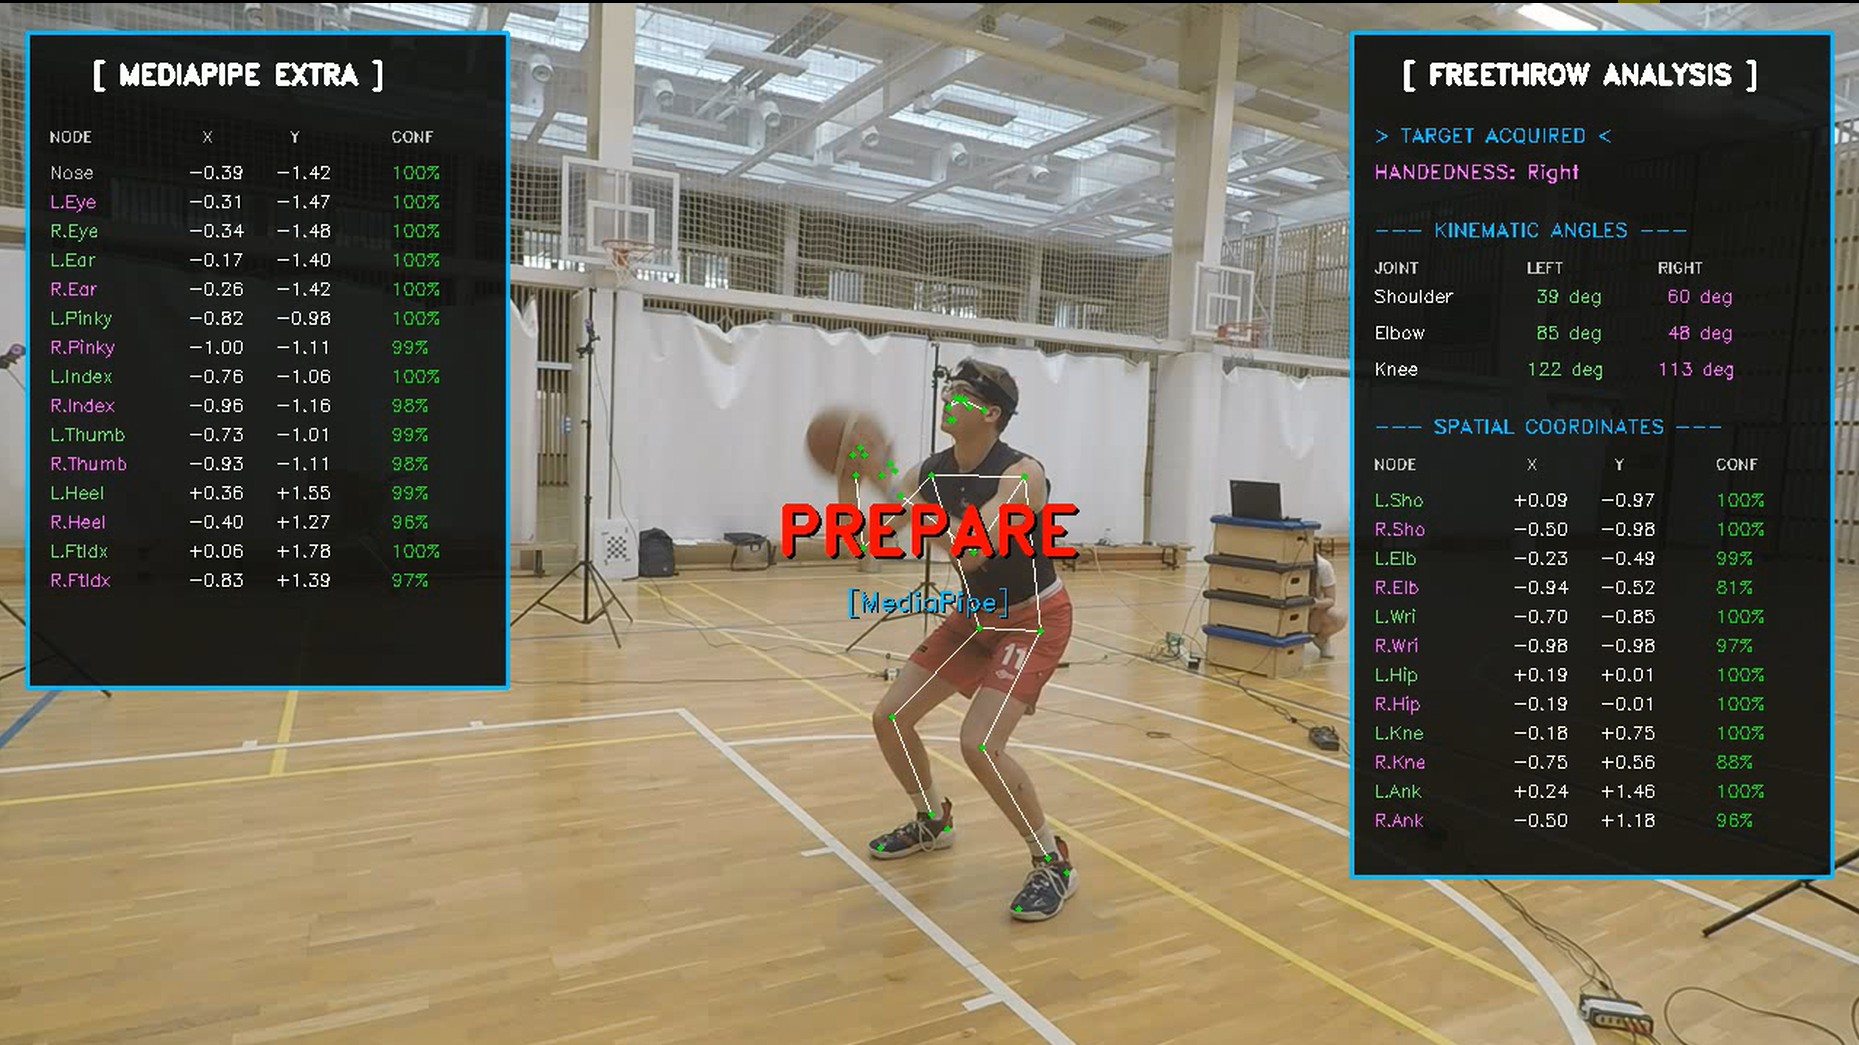
\includegraphics[width=0.9\textwidth, keepaspectratio]{imgs/debug_hud.png}
    \caption{A feldolgozó rendszer által készített vizualizáció, amely valós időben mutatja az azonosított kulcspontokat és az aktuális ízületi szögeket (flexiós és extenziós szögek).}
    \label{fig:debug_hud}
\end{figure}

A \ref{fig:debug_hud}. ábra azt a valós idejű vizualizációt mutatja be, amelyet az adatok ellenőrzésére hoztam létre.

\section{Gépi tanulás}
A kinyert kinematikai adatokból komplex idősoros változókat (features) képeztem. A kulcsízületek (csukló, könyök, váll, csípő, térd, boka) függőleges elmozdulását és ízületi szögeit 30 egyenlő időlépésre (timestep) osztottam fel. Ezen felül olyan másodlagos paramétereket is meghatároztam, mint a csukló mozgástartománya, vagy a csukló sebessége az elengedés pillanatában.

A predikcióhoz együttes tanulási (ensemble) modelleket tanítottam be: a \textit{Random Forest} (Véletlen Erdő) és a \textit{Gradient Boosting} (Gradiens Emelés) algoritmusokat használtam. A modellek megbízhatóságának és általánosító képességének tesztelésére egy 5-szörös keresztvalidációs (StratifiedGroupKFold) módszert alkalmaztam. Ennek az eljárásnak a lényege, hogy egy játékos azonos dobásai (még ha két különböző kamerából is rögzítettük őket) soha nem kerülhettek egyszerre a modell tanítására és tesztelésére használt adatok közé. Ez a szigorú csoportosítás garantálta, hogy nem jött létre adatszivárgás (data leakage), így a validációs pontosság valós képet ad a rendszer teljesítményéről.
